\section{Programming Tool: RViz Teach Panel}

The RViz teach panel is the operator-facing programming tool used in the digital twin workflow. It is important to distinguish it from the operating modes of the twin. The teach panel is not itself a digital twin mode; instead, it is the interface used to create the robot programs that are later validated and executed by the program mode.

The panel was implemented as a custom RViz plugin in the \texttt{dual\_arms\_teach\_panel} package. It allows the operator to select the active robot, define end-effector targets, record waypoints, record gripper commands, save and load programs, and request simulation validation or real execution. This makes RViz more than a visualization environment: it becomes the main teaching station for the digital twin system.

\begin{figure}[H]
    \centering
    \resizebox{\textwidth}{!}{%
    \begin{tikzpicture}[
        font=\small,
        node distance=0.85cm and 1.2cm,
        input/.style={draw, rounded corners=2pt, align=center, minimum width=2.8cm, minimum height=0.85cm, fill=purple!8},
        logic/.style={draw, rounded corners=2pt, align=center, minimum width=3.1cm, minimum height=0.85cm, fill=orange!10},
        data/.style={draw, rounded corners=2pt, align=center, minimum width=2.9cm, minimum height=0.85cm, fill=gray!8},
        mode/.style={draw, rounded corners=2pt, align=center, minimum width=2.9cm, minimum height=0.85cm, fill=green!8},
        arrow/.style={-Latex, thick}
    ]
        \node[input] (marker) {Marker drag};
        \node[input, below=of marker] (servo) {Servo jog};
        \node[input, below=of servo] (manual) {Manual XYZ / RPY};

        \node[logic, right=of servo] (ik) {Teach panel\\pose selection and IK};
        \node[data, right=of ik] (steps) {Waypoints and\\gripper steps};
        \node[data, right=of steps] (yaml) {YAML program\\\texttt{\textasciitilde/.ros/dt\_programs}};

        \node[mode, above right=0.25cm and 1.0cm of yaml] (validate) {Twin validation\\\texttt{/dt/program\_validate}};
        \node[mode, below right=0.25cm and 1.0cm of yaml] (execute) {Real execution request\\\texttt{/dt/program\_execute}};

        \draw[arrow] (marker) -- (ik);
        \draw[arrow] (servo) -- (ik);
        \draw[arrow] (manual) -- (ik);
        \draw[arrow] (ik) -- (steps);
        \draw[arrow] (steps) -- (yaml);
        \draw[arrow] (yaml) -- (validate);
        \draw[arrow] (yaml) -- (execute);

        \begin{scope}[on background layer]
            \node[draw, dashed, rounded corners=4pt, fit=(marker)(servo)(manual)(ik), inner sep=0.28cm, label=above:Teaching interface] {};
            \node[draw, dashed, rounded corners=4pt, fit=(steps)(yaml), inner sep=0.28cm, label=above:Program storage] {};
            \node[draw, dashed, rounded corners=4pt, fit=(validate)(execute), inner sep=0.28cm, label=above:Program mode interface] {};
        \end{scope}
    \end{tikzpicture}%
    }
    \caption{Role of the RViz teach panel in creating programs for the digital twin workflow.}
    \label{fig:dt_teach_panel_workflow}
\end{figure}

\begin{figure}[H]
    \centering
    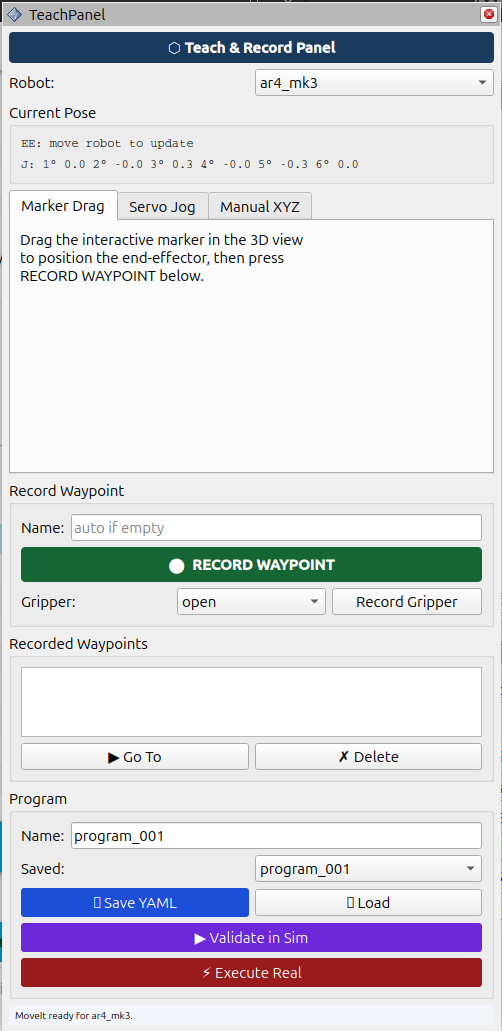
\includegraphics[height=0.78\textheight]{figures/teach_panel.png}
    \caption{RViz teach panel interface used to create and manage digital twin programs.}
    \label{fig:dt_teach_panel_interface}
\end{figure}

\newpage

\subsection{Purpose of the Teach Panel}

The purpose of the teach panel is to provide a practical lead-through programming workflow for the dual-arm cell. Instead of manually writing trajectory files or directly editing joint vectors, the operator can define meaningful robot poses from inside RViz and save them as named program steps.

This is especially useful for collaborative assembly tasks because the required motions are often task-specific. The operator may need to place one arm near a fixture, move the other arm into a handover pose, open or close a gripper, and then repeat the process for another assembly step. The teach panel allows these operations to be captured as an ordered program while keeping the robot model, planning scene, and target markers visible in the same interface.

\subsection{Teaching Methods}

The teach panel supports three methods for defining a target pose. The first method is marker dragging. In this method, the operator moves the interactive marker provided by the MoveIt MotionPlanning display. The panel subscribes to the interactive-marker feedback topic and stores the latest marker pose as the target end-effector pose.

The second method is servo jogging. In this mode, the operator applies incremental Cartesian jog commands. The panel accumulates these increments into a target pose and republishes the updated pose to the RViz marker goal topic. This gives the operator fine control over small pose adjustments while preserving visual feedback in the 3D view.

The third method is manual Cartesian entry. The operator enters position and orientation values directly through the panel. This is useful when the target is known numerically, for example when a fixture location or nominal assembly pose has already been measured.

Together, these three methods make the teaching workflow flexible. Marker dragging is fast for approximate positioning, servo jogging is useful for fine adjustment, and manual entry is useful when exact coordinates are required.

\subsection{Waypoint Recording Through Inverse Kinematics}

When the operator records a waypoint, the panel first determines the active robot and the current target pose. The pose source depends on the selected teaching method: marker feedback, servo jog target, or manual XYZ/RPY input.

The panel then uses MoveIt to solve inverse kinematics for the selected robot. In the implementation, the call to \texttt{setApproximateJointValueTarget} converts the target end-effector pose into a joint-space target for the active planning group. The resulting joint vector is stored in a waypoint structure together with the robot name, waypoint name, timestamp, validation flag, and original end-effector pose.

This design gives the saved program two useful representations of the same step. The joint vector is directly usable by the validation and execution runners, while the end-effector pose preserves the task-space intention of the taught waypoint. Keeping both fields makes the program easier to inspect and debug.

\subsection{Gripper Command Recording}

The teach panel also records gripper commands as program steps. A gripper step stores the active robot, the requested gripper state, the timestamp, and a command type of \texttt{gripper}. The supported gripper states are \texttt{open} and \texttt{closed}.

Treating gripper commands as waypoints in the same ordered list is important for assembly tasks. It allows the program to represent both motion and manipulation in a single sequence. For example, a program can move to an approach pose, close the gripper, move to a placement pose, and then open the gripper. The validation and execution stages can then process the sequence in the same order seen by the operator.

\subsection{YAML Program Storage}

Programs are stored as YAML files by the \texttt{ProgramManager} class. The files are saved in the user's ROS program directory, under \texttt{dt\_programs}, and each saved program is written as a separate \texttt{.yaml} file.

Each program file contains the program name, creation timestamp, global validation flag, and an ordered list of steps. Each step stores its type, name, robot, validation state, timestamp, joint values, end-effector pose, and, when applicable, gripper state. This format is human-readable, easy to inspect during debugging, and simple for the program runners to load.

An abbreviated example of a saved program is shown below. The first entry is a robot motion waypoint, while the second entry is a gripper command in the same ordered sequence.

\newpage

\begin{Verbatim}[fontsize=\small, frame=single]
program_name: pick_and_place_demo
created: 2026-03-11T14:32:01
validated: false
waypoints:
  - id: 1
    type: waypoint
    name: ar4_pick_approach
    robot: ar4_mk3
    validated: false
    timestamp: 2026-03-11T14:32:10
    joints: [0.12, -0.45, 0.78, 0.00, 1.20, -0.10]
    ee_pose:
      x: 0.310
      y: -0.120
      z: 0.240
      qx: 0.0
      qy: 0.0
      qz: 0.0
      qw: 1.0
  - id: 2
    type: gripper
    name: ar4_gripper_closed
    robot: ar4_mk3
    validated: false
    timestamp: 2026-03-11T14:32:15
    gripper_state: closed
    joints: []
\end{Verbatim}

The teach panel marks newly recorded steps as unvalidated. This is deliberate. A taught waypoint is only a requested target until the digital twin validation stage confirms that it can be planned and executed in the simulated environment. Therefore, the YAML file acts as the boundary between teaching and validation.

\subsection{Interface to Program Mode}

The teach panel connects to the program mode through ROS topics. When the operator presses the validation command, the panel saves the current program and publishes the program name on \texttt{/dt/program\_validate}. This request is consumed by the simulation validation runner, which loads the YAML file and checks the program through MoveIt and the twin environment.

When the operator requests real execution, the panel reloads the saved program and checks that all waypoints have been validated. If any step is still unvalidated, execution is blocked at the user interface. If the program is validated, the panel publishes the program name on \texttt{/dt/program\_execute}, allowing the real execution runner to load the file and command the physical controllers.

This makes the teach panel the entry point for program creation, but not the authority that proves a program is safe to run. Its role is to capture operator intent and submit that intent to the digital twin workflow. The validation and execution mode, described in the next section, is responsible for testing the saved program and enforcing the validation-before-execution rule.
